%
% $RCSfile: schemes.tex,v $
%
% Copyright (C) 2002-2008. Christian Heller.
%
% Permission is granted to copy, distribute and/or modify this document
% under the terms of the GNU Free Documentation License, Version 1.1 or
% any later version published by the Free Software Foundation; with no
% Invariant Sections, with no Front-Cover Texts and with no Back-Cover
% Texts. A copy of the license is included in the section entitled
% "GNU Free Documentation License".
%
% http://www.cybop.net
% - Cybernetics Oriented Programming -
%
% http://www.resmedicinae.org
% - Information in Medicine -
%
% Version: $Revision: 1.1 $ $Date: 2008-08-19 20:41:08 $ $Author: christian $
% Authors: Christian Heller <christian.heller@tuxtax.de>
%

\subsection{Schemes}
\label{schemes_heading}
\index{Schemes of Terminology}

One of the -- if not the most complex domain in which terminologies are applied
is \emph{Healthcare}. As announced in section \ref{example_heading}, it will
serve as example domain for many ideas presented in this work -- so for this
section describing various organisation schemes for terminologies. The later
chapter \ref{res_medicinae_heading} will come back to this topic once more and
briefly introduce a number of terminology systems for healthcare. Jeremy Rogers
writes about health terminology \cite{rogers2002}:

\begin{quote}
    Health terminology is complex and multifaceted, more so than most language
    domains. It has been estimated that between 500,000 and 45 million different
    concepts are needed to adequately describe concepts like conditions of
    patients and populations, actions in healthcare and related concepts, such as
    biomedical molecules, genes, organisms, technical methods and social concepts.

    The system itself can, for example, be called an ontology, medical entity
    dictionary, coding- and reference model or reference terminology. The
    differences in terminology are understandable -- this kind of work is highly
    interdisciplinary and integrates knowledge from linguistics, philosophy,
    informatics and health sciences, and there is room for misunderstanding
    between disciplines.
\end{quote}

After him \cite{rogers}, there were three broad families of technical approaches
to terminologies: \emph{Enumerative Scheme}, \emph{Compositional Scheme} and
\emph{Lexical Scheme}. These are explained in the following subsections, mostly
citing freely after Rogers \cite{rogers}. The language defined in chapter
\ref{cybernetics_oriented_language_heading} might possibly be suitable for
creating terminologies following an enumerative- or, better yet, compositional
scheme.

%
% $RCSfile: enumerative_scheme.tex,v $
%
% Copyright (C) 2002-2008. Christian Heller.
%
% Permission is granted to copy, distribute and/or modify this document
% under the terms of the GNU Free Documentation License, Version 1.1 or
% any later version published by the Free Software Foundation; with no
% Invariant Sections, with no Front-Cover Texts and with no Back-Cover
% Texts. A copy of the license is included in the section entitled
% "GNU Free Documentation License".
%
% http://www.cybop.net
% - Cybernetics Oriented Programming -
%
% http://www.resmedicinae.org
% - Information in Medicine -
%
% Version: $Revision: 1.1 $ $Date: 2008-08-19 20:41:06 $ $Author: christian $
% Authors: Christian Heller <christian.heller@tuxtax.de>
%

\subsubsection{Enumerative Scheme}
\label{enumerative_scheme_heading}
\index{Enumerative Scheme}
\index{Enumerative Coding Scheme}
\index{Taxonomic Classification}
\index{International Classification of Diseases}
\index{ICD}

An \emph{Enumerative Coding Scheme} lists, within the scheme, \emph{all} phrases
ever to be used, and gives each of them its own code for reference. The phrases
can be very long and detailed. The list of phrases provided is \emph{finite},
and it is \emph{fixed}.

\begin{table}[ht]
    \begin{center}
        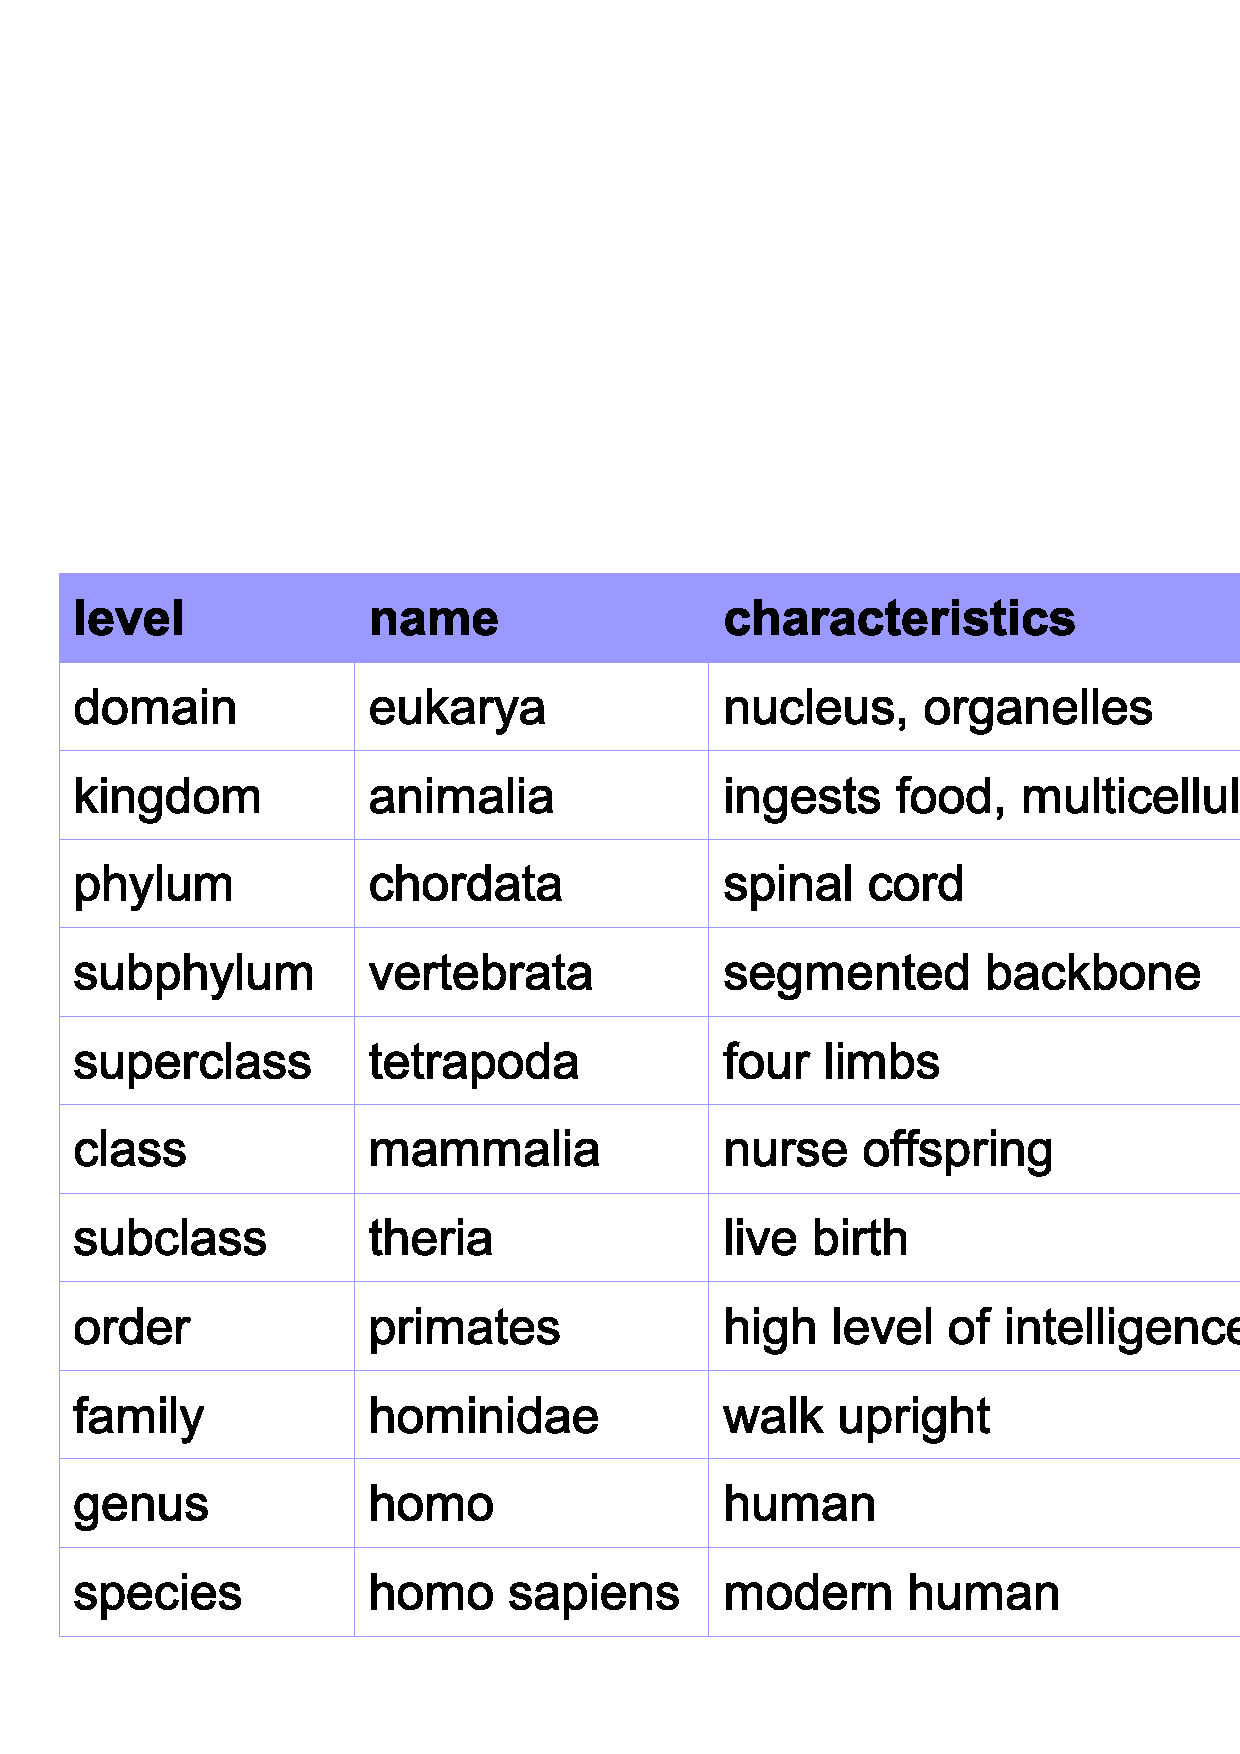
\includegraphics[scale=0.4,angle=-90]{graphic/taxonomy.pdf}
        \caption{Taxonomic Classification of the Animal Kingdom}
        \label{taxonomy_table}
    \end{center}
\end{table}

A very familiar example of an enumerated scheme is the traditional taxonomic
classification of the animal kingdom (figure \ref{taxonomy_table}). Most of the
existing medical terminologies, listing names of diseases, of surgical
operations and the like, are also enumerative. One example is the
\emph{International Classification of Diseases} (ICD) (chapter
\ref{res_medicinae_heading}).

After \cite{rogers}, attempting to enumerate in advance all useful phrases
inevitably encounters two serious problems concerning the \emph{Scale} and
\emph{Organisation}. Terminologies become:

\begin{enumerate}
    \item \emph{Scale:} too big to maintain, which results in inconsistent data
        that cannot be analysed anymore
    \item \emph{Organisation:} pre-categorised, which does not allow terms to
        be simultaneously placed under all different categories that are valid
\end{enumerate}

A further limitation is caused by unfavourable technical choices. The code often
serves two purposes. It is: the unique identifier of a concept and the means of
representing the relative organisation of a concept. So the common practice of
restricting the physical length of a code also restricts the levels of
organisation.

%
% $RCSfile: compositional_scheme.tex,v $
%
% Copyright (C) 2002-2008. Christian Heller.
%
% Permission is granted to copy, distribute and/or modify this document
% under the terms of the GNU Free Documentation License, Version 1.1 or
% any later version published by the Free Software Foundation; with no
% Invariant Sections, with no Front-Cover Texts and with no Back-Cover
% Texts. A copy of the license is included in the section entitled
% "GNU Free Documentation License".
%
% http://www.cybop.net
% - Cybernetics Oriented Programming -
%
% http://www.resmedicinae.org
% - Information in Medicine -
%
% Version: $Revision: 1.1 $ $Date: 2008-08-19 20:41:06 $ $Author: christian $
% Authors: Christian Heller <christian.heller@tuxtax.de>
%

\subsubsection{Compositional Scheme}
\label{compositional_scheme_heading}
\index{Compositional Scheme}
\index{Compositional Conceptual Scheme}
\index{Dictionary}
\index{Generalised Architecture for Languages, Encyclopedias and Nomenclatures in Med.}
\index{GALEN}
\index{Systematized Nomenclature of Medicine}
\index{SNOMED}
\index{Enumerative-compositional Scheme}
\index{Logical Observation Identifiers, Names and Codes}
\index{LOINC}
\index{International Classification of Nursing Procedures}
\index{ICNP}
\index{Combinatorial Explosion}

A \emph{Compositional Conceptual Scheme} typically contains a \emph{controlled}
and \emph{fixed} list (\emph{Dictionary}) of a relatively small number (a few
ten-thousand) of \emph{primitive} terms, each of which can have a unique code.
These primitives may be combined together by users to form more complex terms,
including those which might be found in an existing enumerative scheme but also
other, sometimes trivial, variations and expansions \cite{rogers}.

Examples of compositional schemes include the \emph{Generalised Architecture
for Languages, Encyclopaedias and Nomenclatures in Medicine} (GALEN) and the
\emph{Systematized Nomenclature of Medicine} (SNOMED). Hybrid
enumerative-compositional schemes are
\emph{Logical Observation Identifiers, Names and Codes} (LOINC) and the
\emph{International Classification of Nursing Procedures} (ICNP).

The sheer unlimited number of possible combinations, when seen as a problem, is
called \emph{Combinatorial Explosion}. Much worse problems, however, are the:

\begin{itemize}
    \item[-] \emph{Nonsense} combinations that may be constructed
        (avoidable with a set of semantic links, a grammar and constraints)
    \item[-] \emph{Redundancy} which occurs when more than one combination of
        terms express the same concept
        (avoidable with formal algorithms helping to identify redundant compositions)
    \item[-] \emph{Post-hoc Classification} (unforeseeable addition of new,
        unknown concepts) that may prevent a meaningful data analysis
        (avoidable with a type hierarchy of primitives and of semantics links)
    \item[-] \emph{Intractability} of data due to \emph{exploding} computer
        algorithms so that the computer will never find an answer
\end{itemize}

%
% $RCSfile: lexical_scheme.tex,v $
%
% Copyright (C) 2002-2008. Christian Heller.
%
% Permission is granted to copy, distribute and/or modify this document
% under the terms of the GNU Free Documentation License, Version 1.1 or
% any later version published by the Free Software Foundation; with no
% Invariant Sections, with no Front-Cover Texts and with no Back-Cover
% Texts. A copy of the license is included in the section entitled
% "GNU Free Documentation License".
%
% http://www.cybop.net
% - Cybernetics Oriented Programming -
%
% http://www.resmedicinae.org
% - Information in Medicine -
%
% Version: $Revision: 1.1 $ $Date: 2008-08-19 20:41:07 $ $Author: christian $
% Authors: Christian Heller <christian.heller@tuxtax.de>
%

\subsubsection{Lexical Scheme}
\label{lexical_scheme_heading}
\index{Lexical Scheme}
\index{Lexical Tech}
\index{Unified Medical Language System}
\index{UMLS}

A \emph{Lexical Technique} is one that helps compare phrases based on what they
appear to say -- on which words appear, in which order, and in what grammatical
constructs -- rather than on what they might or might not actually mean. Such
techniques can provide a powerful (but not 100\% accurate) method for mapping
between phrases in existing schemes, or between such phrases and the text found
in papers, the \emph{World Wide Web} (WWW) or other electronic resources.

One example of a lexical scheme is the \emph{Unified Medical Language System}
(UMLS).

Where lexical techniques break is when the language gets more \emph{slippery},
that is ambiguities may occur. Humans might interpret such results correctly,
but automated decision support systems would fail. Rogers \cite{rogers}
concludes that: \textit{As an input for autonomous machine processing
applications such as decision support, the outputs of natural language
processing tools remain unsuitable.}

